\documentclass{article}
\usepackage[utf8]{inputenc}
\usepackage{graphicx}

\title{Resume Artificial Intellegent}
\author{Dimas Aqila Maulana - 1184081}


\begin{document}

\maketitle
\section{Kecerdasan Buatan}
\subsection{Definisi Kecerdasan Buatan}
 \hspace{1cm} Kecerdasan buatan yakni kecerdasan yang ditambahkan pada suatu sistem yang bisa diatur dalam konteks ilmiah disebut juga  intelegensi artifisial atau AI, mempunyai definisi sebagai kecerdasan entitas ilmiah. Andreas Kaplan dan Michael Haenlein sendiri menafsirkan kecerdasan buatan sebagai “kemampuan sistem untuk menafsirkan data eksternal dengan benar, untuk belajar dari data tersebut, dan menggunakan pembelajaran tersebut guna mencapai tujuan dan tugas tertentu melalui adaptasi yang fleksibel”. Sistem seperti ini umumnya dianggap komputer. Kecerdasan dibuat dan dimasukkan ke dalam suatu mesin (komputer) agar bisa melakukan pekerjaan seperti halnya yang dilakukan manusia. Berbagi macam bidang yang memakai kecerdasan buatan contohnya sistem pakar, permainan komputer (games), logika fuzzy, jaringan saraf tiruan dan robotika dan lain-lain.
 
\hspace{1cm}Contoh  implementasi  AI  sebagai  penggunaan teknologi informasi adalah cloud computing yang disajikan berdasarkan utilitas secara on demand.Cloud computing sebenarnya  bukanlah  hal  yang  baru  dalam dunia   teknologi informasi. Web   service, internet service provider(ISP), programmable web,   dan virtualisasi   merupakan   konsep-konsep   yang   telah berkembang   dan   memberi   kontribusi   pada   evolusi teknologi ini. Beberapa definisi mengenai konsep cloud computingtelah   sering   dikemukakan   diberbagai literatur.

\subsection{Sejarah dan perkembangan Kecerdasan Buatan}
\hspace{1cm} McMulloh dan Pitts pada tahun 1943 mengusulkan model matematis bernama perceptron dari neuron di dalam  otak.  Mereka juga menunjukkan  bagaimana neuron menjadi aktif seperti saklar on-off dan neuron tersebut mampu untuk belajar dan memberikan aksi berbeda terhadap waktu dari input yang diberikan.  Sumbangan terbesar di bidang AI diawali pada paper Alan Turing, pada tahun 1950 yang mencoba menjawab  “Dapatkah computer berfikir” dengan menciptakan mesin Turing.  Paper Alan Turing pada tahun 1950 berjudul “Computing Machineri and Intelligence” mendiskusikan syarat sebuah mesin dianggap cerdas. Dia beranggapan bahwa jika mesin dapat dengan sukses berprilaku seperti manusia, kita dapat menganggapnya cerdas.

\hspace{1cm} Pada akhir 1955, Newell dan Simon mengembangkan  The Logic Theorist, program AI pertama. Program ini merepresentasikan  masalah sebagai model pohon, lalu penyelesaiannya dengan  memilih cabang yang akan menghasilkan kesimpulan terbenar. Program ini berdampak besar dan menjadi batu loncatan penting dalam mengembangkan bidang AI. Pada tahun 1956 John McCarthy dari  Massacuhetts Institute of Technology dianggap sebagai bapak AI, menyelenggarakan konferensi untuk menarik para ahli komputer bertemu, dengan  nama kegiatan “The Dartmouth summer research project on artificial intelligence.” 

\subsection{Supervised learning dan Unsupervised Learning}
\hspace{1cm} Supervised learning adalah algoritma yang paling sering digunakan dalam dunia data science dibandingkan dengan unsupervised learning. Analisis regresi linier berganda maupun logistik yang notabene sudah tidak asing lagi di dengar adalah salah satu contoh dari supervised learning. Perbedaan kedua algorima tersebut terletak pada bagaimana mereka belajar untuk membuat suatu prediksi maupun klasifikasi. Dalam supervised learning, algoritma tersebut seolah-olah dilatih terlebih dahulu agar dapat melakukan prediksi maupun klasifikasi.

\hspace{1cm} Unsupervised Learning tidak menggunakan data latih atau data training untuk melakukan prediksi maupun klasifikasi. Berdasarkan model matematisnya, algoritma ini tidak memiliki target variabel. Salah satu tujuan dari algoritma ini adalah mengelompokkan objek yang hampir sama dalam suatu area tertentu. Contoh dari penerapan metode ini adalah ketika seorang data analyst ingin mengelompokkan customer salah satu provider hosting Indonesia berdasarkan kemiripan sifat dalam hal pendapatan, umur, hobi, dan jenis pekerjaan.

\subsection{Data Set, Training Test, Testing Test}
\hspace{1cm} Berbicara mengenai Supervised learning serta unsupervised learning maka harus adanya pembahasan mengenai definisi dataset. Dataset adalah kumpulan sampel yang sudah dikumpulkan. Seorang anak ingin bermain badminton, tetapi keputusannya untuk bermain badminton (play) tergantung pada variable yang ditentukan contohnya jarak kaki dari gairs dan atau tinggi net sehingga variable varibale ini disebut fitur.

\hspace{1cm} Sedangkan Training set adalah bagian dataset yang kita latih untuk membuat prediksi atau menjalankan fungsi dari sebuah algoritma ML. Kita memberikan petunjuk melalui algoritma agar mesin yang kita latih bisa mencari korelasinya sendiri atau belajar pola dari data yang diberikan.Testing Test adalah bagian dataset yang kita tes untuk melihat keakuratannya, atau dengan kata lain melihat performanya.


\section{Instalasi}
\begin{enumerate}
    \item Instalasi library scikit dari anaconda dengan pip install -U scikit-learn
     \begin{center}
    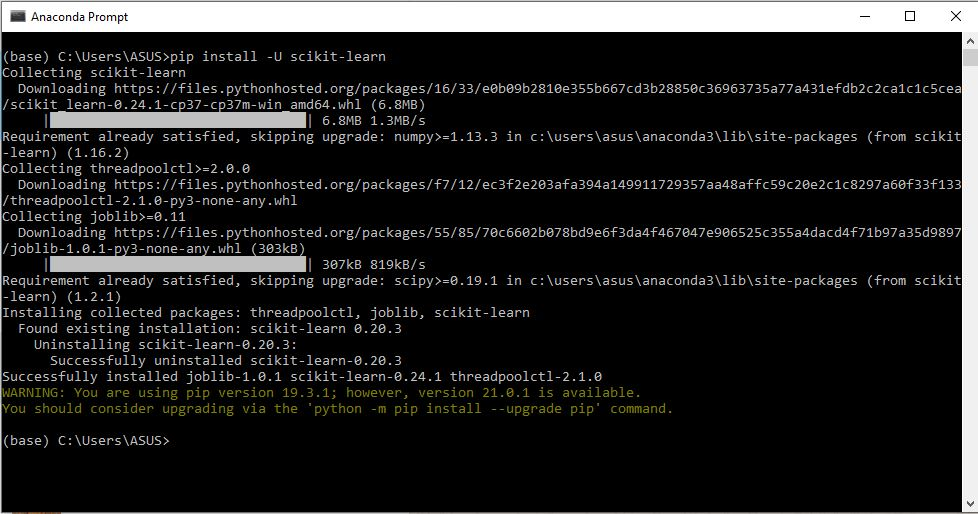
\includegraphics[width=.8\textwidth]{1184081/chapter1/Capture1.JPG}
    \end{center}
    \item Mencoba Loading dan example dataset.
    \begin{center}
    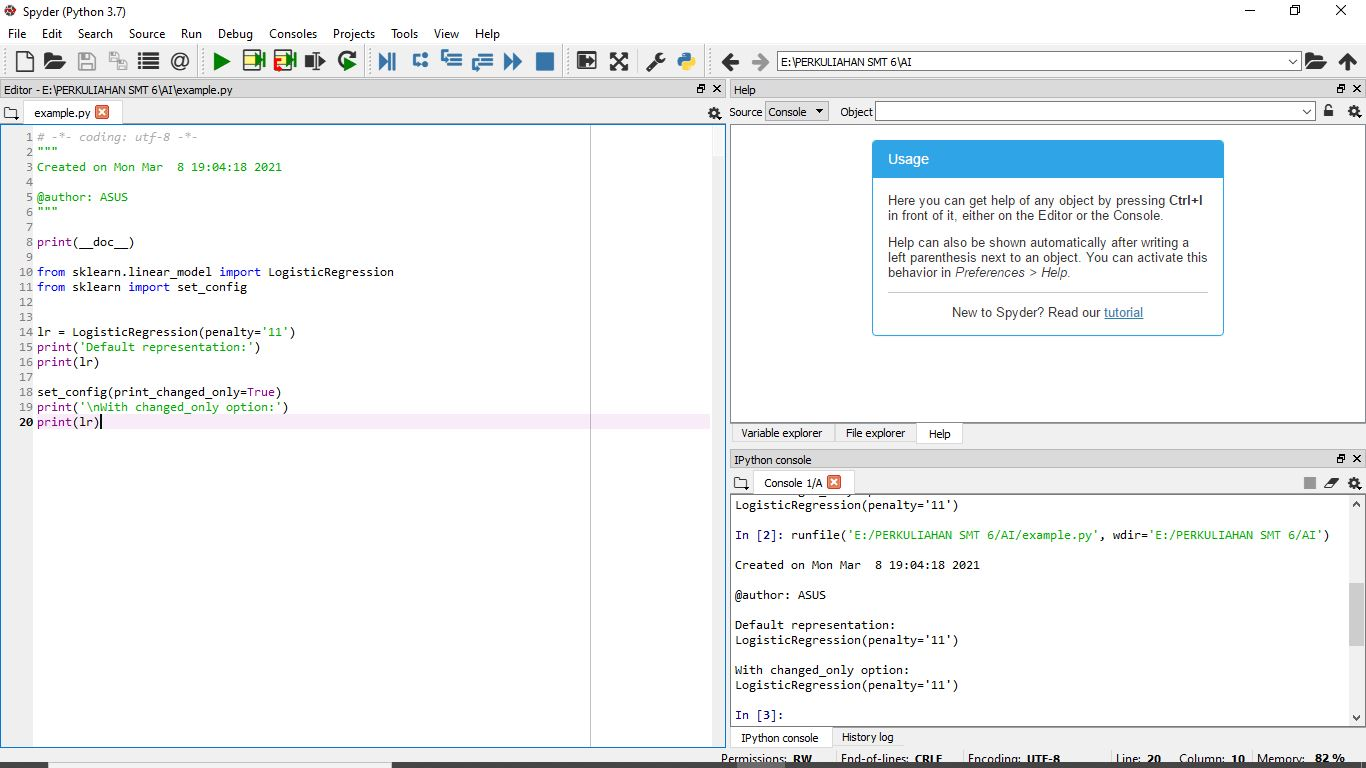
\includegraphics[width=.8\textwidth]{1184081/chapter1/Capture2.JPG}
    \end{center}
     \begin{center}
    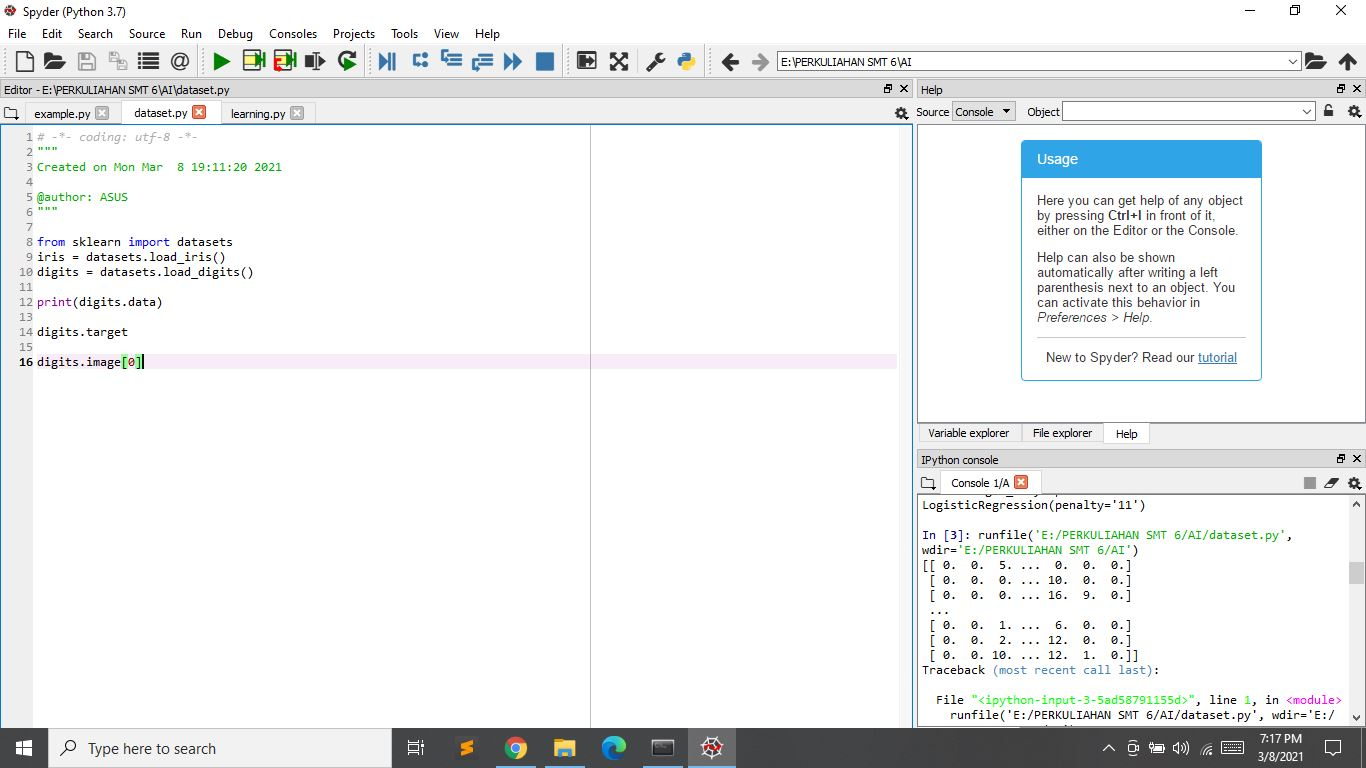
\includegraphics[width=.8\textwidth]{1184081/chapter1/Capture3.JPG}
    \end{center}
    \item Mencoba Learning and predicting.
    \begin{center}
    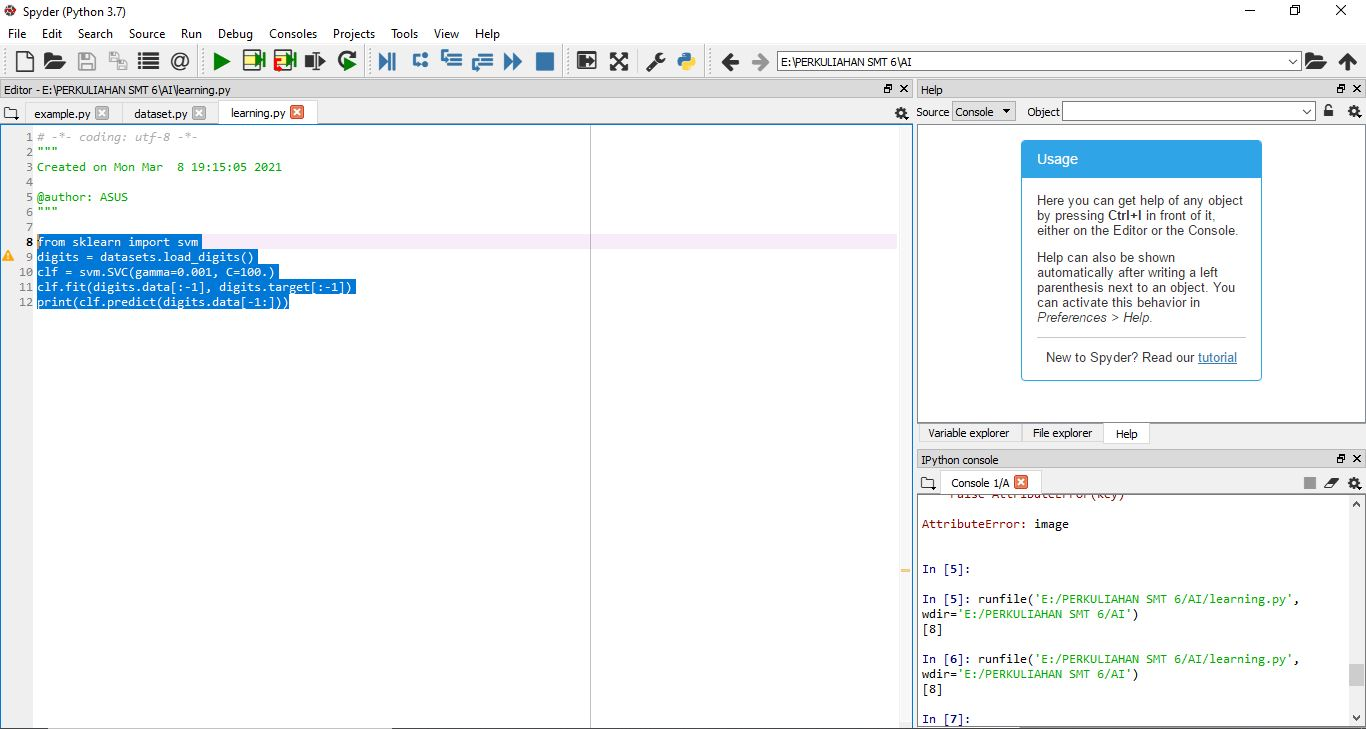
\includegraphics[width=.8\textwidth]{1184081/chapter1/Capture4.JPG}
    \end{center}
    \item Mencoba Model persistence
    \begin{center}
    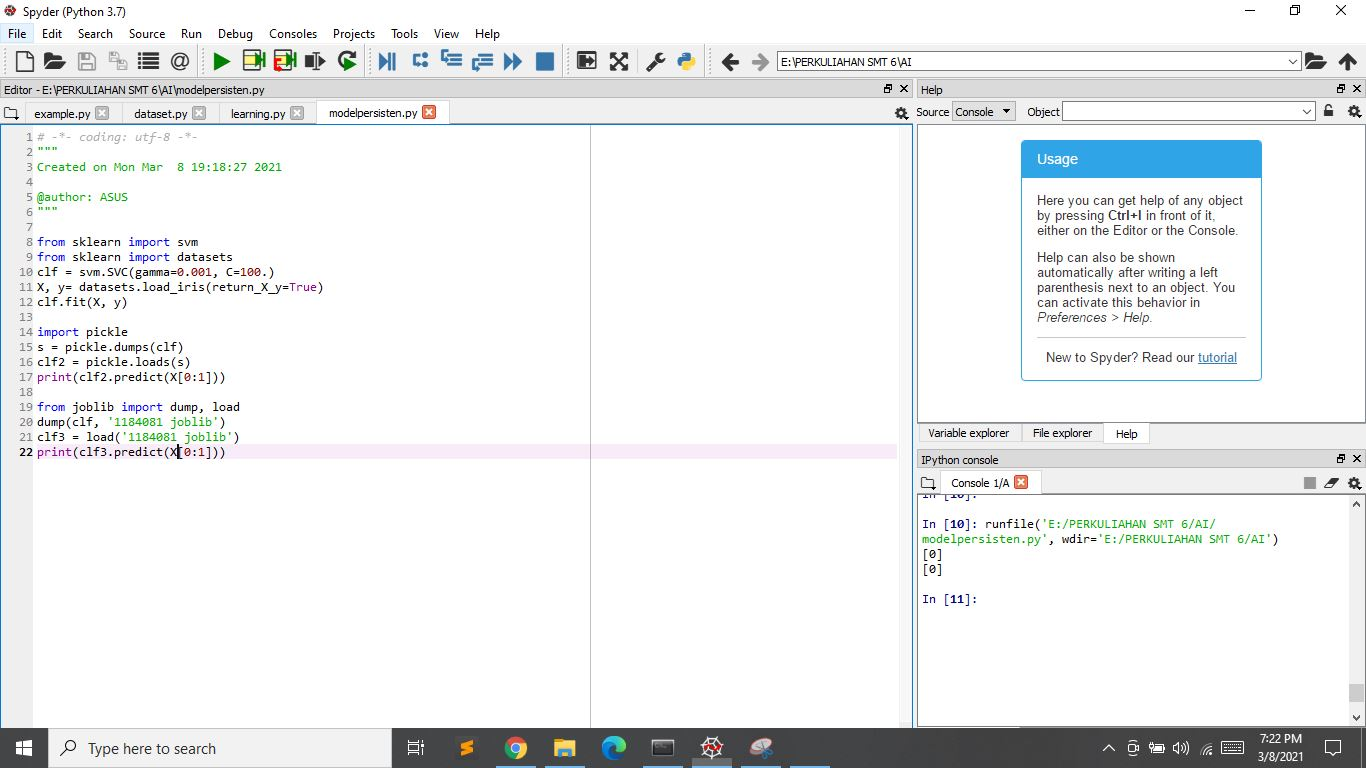
\includegraphics[width=.8\textwidth]{1184081/chapter1/Capture5.JPG}
    \end{center}
    \item Mencoba Conventions.
     \begin{center}
    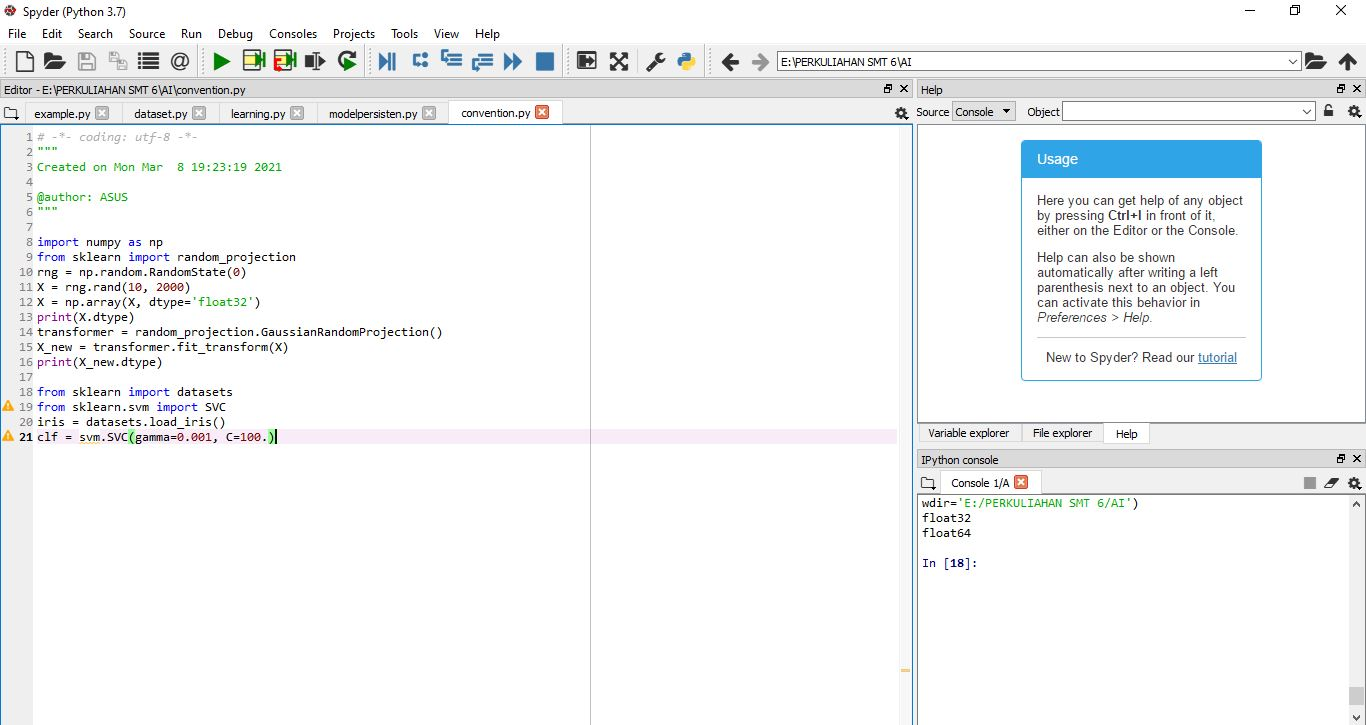
\includegraphics[width=.8\textwidth]{1184081/chapter1/Capture6.JPG}
    \end{center}
    \item Hasil Model persistence
     \begin{center}
    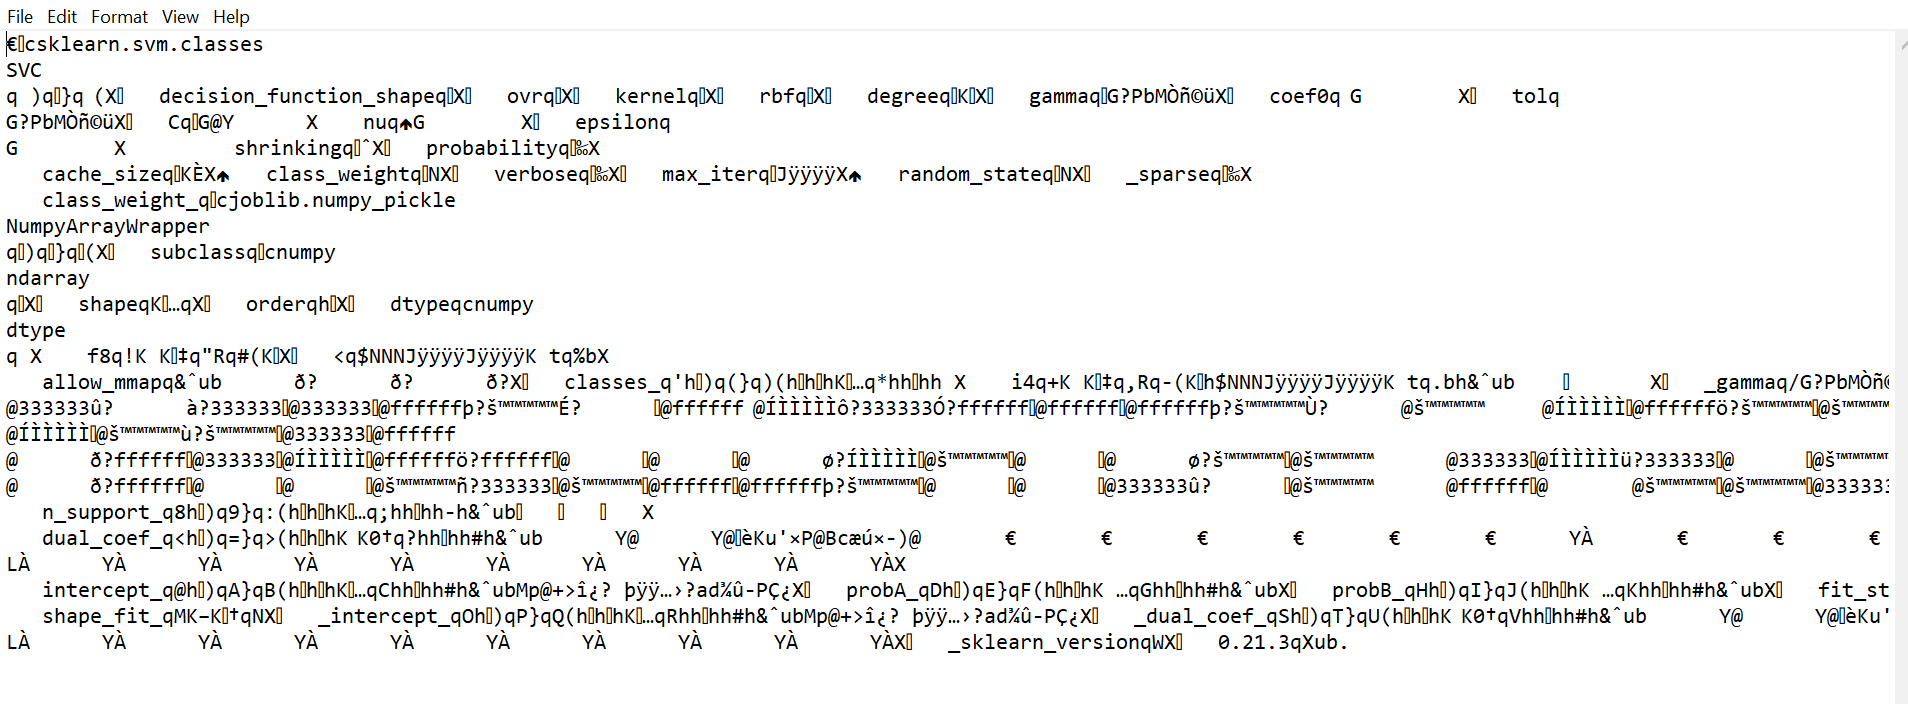
\includegraphics[width=.8\textwidth]{1184081/chapter1/Capture7.PNG}
    \end{center}
\end{enumerate}

\section{Error dan Penanganannya}
\begin{enumerate}
    \item Terdapat error dalam Dataset.py yaitu SyntaxError: invalid syntax
      \begin{center}
    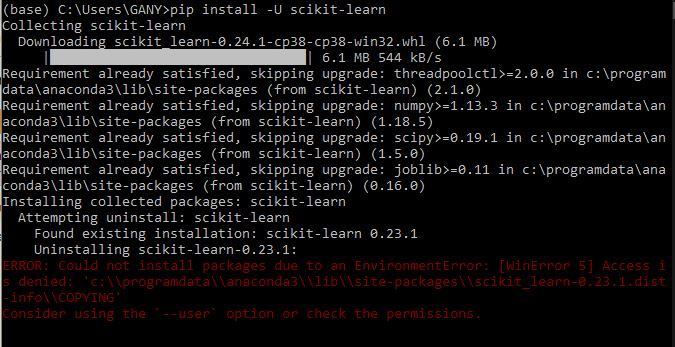
\includegraphics[width=.8\textwidth]{1184081/chapter1/error1.JPG}
    \end{center}
    \\
    penangananya adalah harus menghapus tanda kurung disamping datasets.
     \begin{center}
    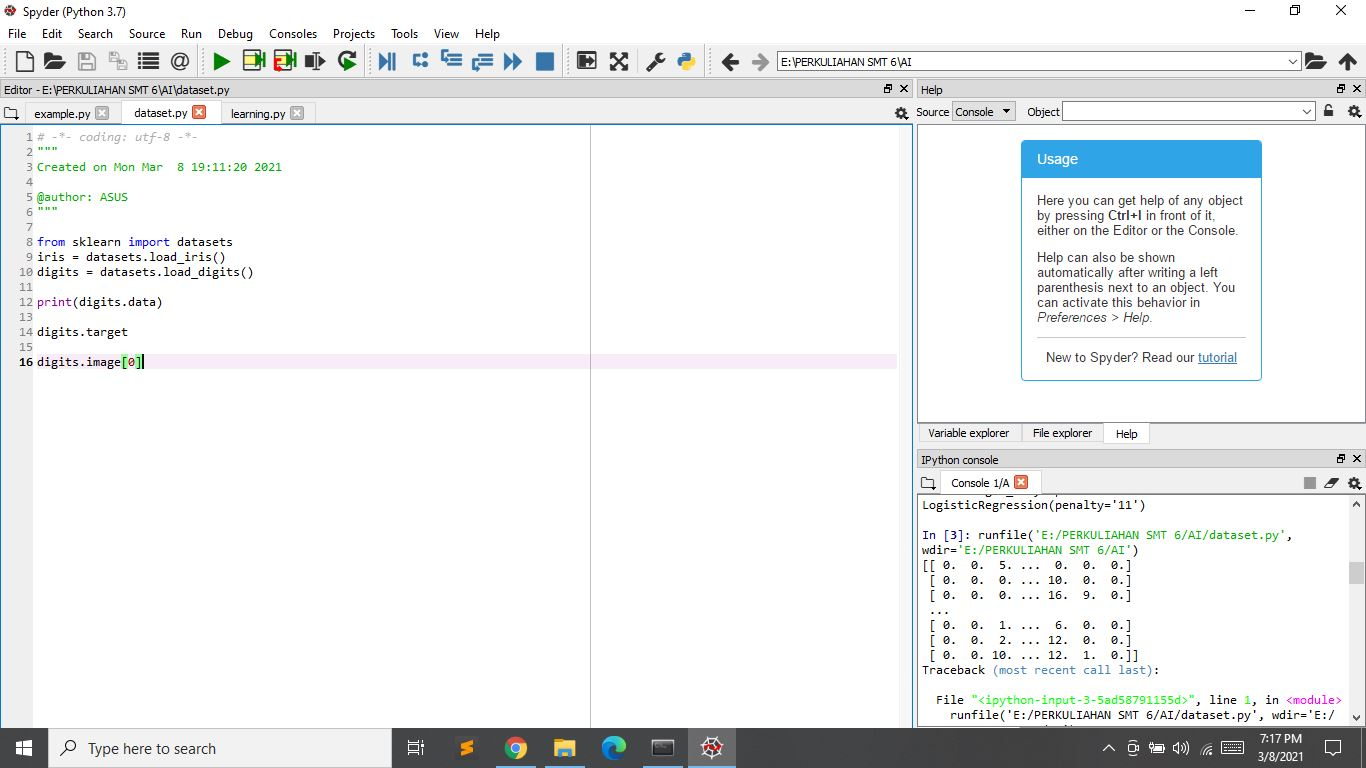
\includegraphics[width=.8\textwidth]{1184081/chapter1/Capture3.JPG}
    \end{center}
    \item Terdapat error dalam Modelpersisten.py name 'x' is not defined.
      \begin{center}
    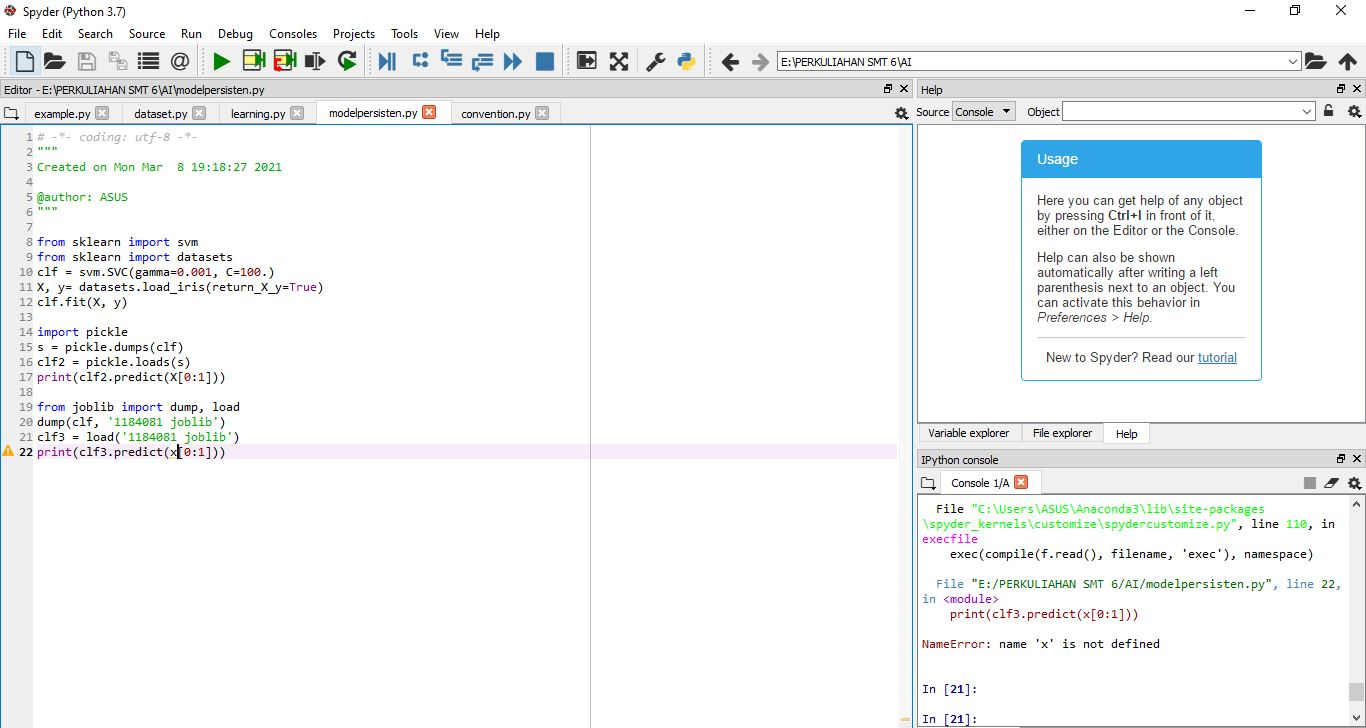
\includegraphics[width=.8\textwidth]{1184081/chapter1/error2.JPG}
    \end{center}
    \\penangananya adalah harus mengubah x yang ada di baris ke 22 menjadi X besar.
     \begin{center}
    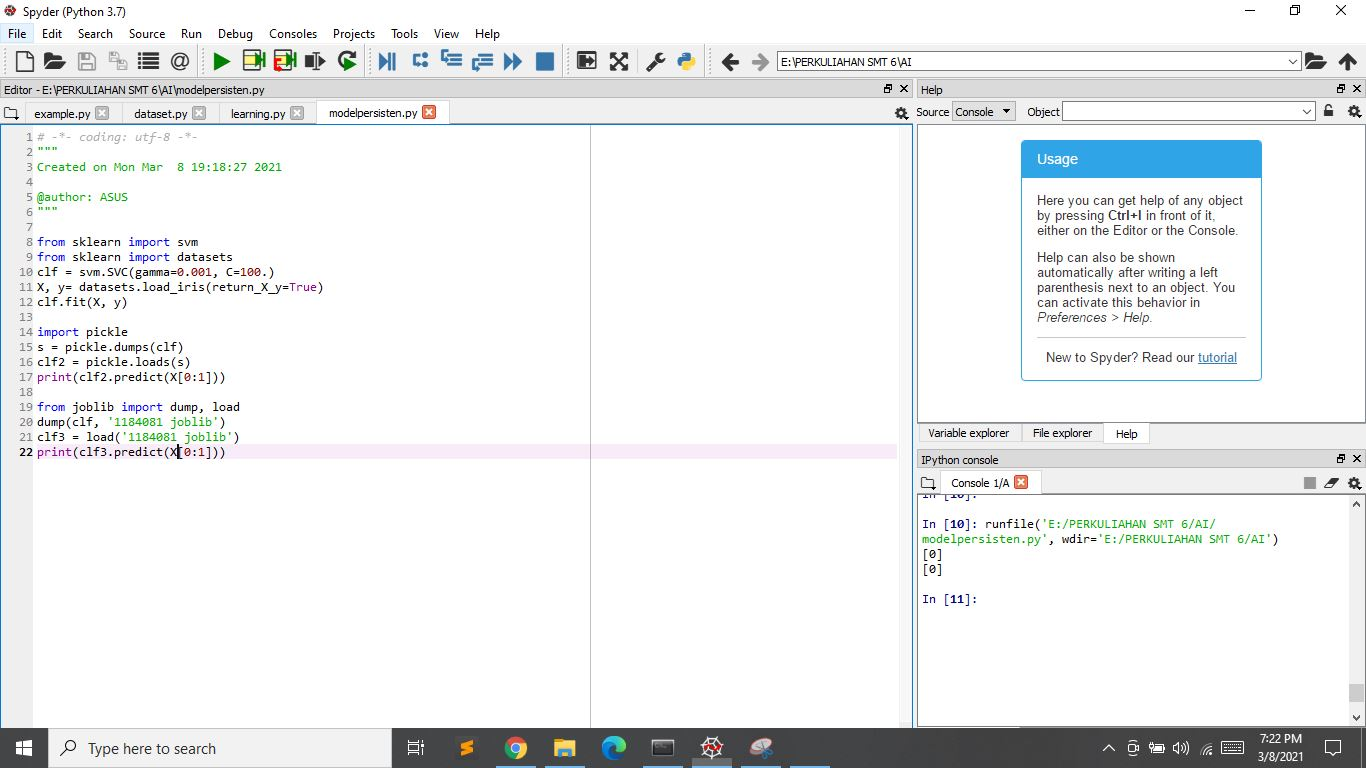
\includegraphics[width=.8\textwidth]{1184081/chapter1/Capture5.JPG}
    \end{center}

\end{enumerate}




\end{document}
